\section{Analysis} \label{sec:analysis}
The purpose of this analysis is to collect the relevant research and data which was deemed necessary during the naïve design phase. This research is going to be used as a basis for a prototype, which should help us answer our problem statement. 

\subsection{Product Comparisons}
As stated by our initial problem, can an ordinary webcam compare to other gaming platforms? It is necessary to figure out which other gaming platforms to compare the webcam with. Since the webcam is a video camera it can be easily be compared with other video game platforms that utilize a video camera. The Xbox Kinect from Microsoft utilizes one RGB-camera and two 3D depth sensors to detect gestures made by the user \parencite{Cong}. The Kinect is popular, having sold roughly 24 million sensors during its current lifespan \parencite{MSByNumbers}, and because it has become such a household name, makes it a suitable platform for comparison.
\bigskip

Another popular brand is the Wii by Nintendo. The Wii was introduced in 2006 and was the first console to have motion control. During its lifespan the Wii has sold near 100 million units worldwide \parencite{NintendoSales}. The Wii also uses a camera but not in the same way as the Microsoft Kinect, instead of using a static VGA camera like the Kinect, the Wii uses an infrared camera positioned within the hand-held controller held by the user to detect the position of the controller in relation to the monitor \parencite{Castaneda2006}. This makes the controller usable as a pointing device. The Wii controller also uses motion sensors to detect the tilting of the controller, which allows the controller to be used as a virtual golf club or tennis racket. The Wii's use of camera technology, makes it suitable for comparison.
\bigskip

The PlayStation Move by Sony was introduced as an add-on to the PlayStation 3 in 2010. The Move uses a video camera in conjunction with motion sensors in a hand-held controller to detect the users position in the 3D space \parencite{Kumar2009}. The move works in many ways as the Nintendo Wii except for the use of camera technology, the Move controller has a visible light on the top of the controller which the camera uses to pinpoint the location of the controller. While the Move is not as popular as the two other products, having sold around 15 million units so far \parencite{Yin-Poole2012}, its use of the camera solution makes it usable for a comparison.

\subsection{State of the art}
To gather knowledge about the process of developing a gaming device using visual computing, the first logical step is to research the "State of the Art", I.e. what have already been done, and how it has been done.

As the problem statement of this report revolves around using a webcam to control a game, it is natural to look at the most dominant solutions on the market, i.e. the Microsoft Xbox 360 Kinect, the PlayStation Move and the Nintendo Wii which will be described the following sections.

The purpose of this research is to gain an understanding of how the team behind the Kinect approached the problem of creating visual computing software, suitable for games, and what they did to solve it, in order to learn from their mistakes and, more importantly, their solutions.

\subsubsection{Development of the Kinect}
\subsubsection*{Kinect}
The Microsoft Xbox 360 Kinect is one of the most successful applications of computer-visual interaction made available to regular consumers of recent years, as proved by the sheer number of sold units during the first 60 days with over 8 million, making it the fastest-selling consumer-electronics device in history \parencite{Knies}.

As the Kinect is probably the most well-known visual computing device for gaming, and it is the device most closely resembling a possible product described by the problem statement, it seems logical to start by researching this.

\subsubsection*{Development:}
At the onset of development, the Xbox development team were using an algorithm that tracked a user's body movement, and used this string of information to 'predict' the movement. Not only were this method a bit unreliable ,it simply couldn't keep up, at times, it was also prone to 'overloading' \parencite{Knies}, even if the algorithm could keep up with the speed of the movement, the tracking would become increasingly more inaccurate over time, and eventually crash, requiring a reset, thus making it unusable for extended game play.

\subsubsection*{Changing the approach:}
The team realized, that they had to change their approach, in order for the application to be suited for video gaming. They figured that as the algorithm crumbled due to it trying to interpret movement from a sequence and therefore trying to predict movement, rather than record it, they needed to change their approach to calculating the movement. \textit{“We couldn’t rely exclusively on context, your history, or your motion in the past. "We realized that we had to look at a single image at a time (...) We had to just look at an image and decide what your body pose was. We knew that this was, in theory, possible, because a person can do this. If you look at a photo, you can draw the position of the joints.”} - Jamie Shotton, 2011.

So instead of trying to predict something as unpredictable as human movement during games, the team figured that the application needed to interpret movement from every frame of a video stream instead - i.e. they needed an algorithm capable of reading a body's position in space from an image, converting said position into data of movement.

Research in this specific field already existed in the computer-vision literature, which made the approach seem promising.

\begin{figure}[h] 
\centering
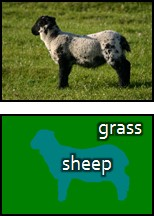
\includegraphics[scale=1]{Sheep1} 
\caption{Sheep-and-grass example.}
\label{fig:Sheep}
\end{figure}
\bigskip

The initial algorithm attempted to match the entire body at once, comparing the image with an extensive database of possible body poses - in essence, the algorithm recorded the body's pose, compared them with the entire library, until it found the best match.

To some extend, the method was functional, but it wasn't going to be efficient enough for the needs of a gaming hardware - As the algorithm checked the entire body at once, it meant that the library had to represent every possible combination of poses, meaning that the library would grow exponentially, causing it to be way too extensive. \parencite{Knies}
The team looked at the existing literature for answers, and found a way to solve the issue:

They had to break up the body into multiple different focus points - i.e. instead of labeling the entire body, they had to identify and label each joint separately.

The way they did this, was to use the "sheep-and-grass" example:
Using an image of a sheep on a grass field, the process isolates the sheep from the grass, automatically labeling the two as sheep and grass, respectively  (fig. \ref{fig:Sheep}).
\bigskip

This principle was used for the Kinect, to label and color parts of a body. Once completed and combined with the gray-scale image from the camera, it was and possible to locate each joint of the body, as the colored parts are defined as being near a joint. By combining the color code of a joint, and the depth information from the gray-scale image, it was possible to estimate the 3D XYZ coordinates of the joint.

\subsubsection*{The Kinect comes to life}
With the object-recognition approach showing promise, the Xbox team started considering how to implement the algorithm on the Xbox 360 hardware, which, at the time, was already three years old. The team needed to figure out a way to implement the tracking algorithm into the existing hardware, taking the ever more demanding games into account.

To solve this, the team used machine learning, and to do this, they needed data.	
\bigskip

\textit{“Mat would feed that motion-capture data into a computer-graphics tool that generated depth images so we’d have something to test on where we knew the right answer. We had a ground-truth answer associated with each image.”} - Fritzgibbon, 2011.
\bigskip

Instead of taking images of real-life people and labeling by hand - a method which is both extremely inefficient and expensive - the team decided to synthesize images, by using computer graphics. After some initial issues with speed or reliability, the team figured out a way to generate the synthesized depth images, which enabled the team to generate millions of images, expanding the training library greatly.

The team then needed to tweak the algorithm to gain greater accuracy, expanding the training library as they went. One problem became apparent, however: it took a very long time to 'train' the program, making the application slow and cumbersome. Using an algorithm dubbed Exemplar ,an algorithm used for object removal and labeling in digital images, \parencite{Cheng2005}, they solved this issue, enabling the application to work fast and accurately enough to run on every single frame of the data-stream of the Kinect depth camera.

Once this was up and running, the team further tweaked the algorithm, enabling them to turn the application to provide a full skeleton, instead of joints, to provide temporal coherence.

By the time the algorithm had been completed, it was capable of processing 30 frames per second, using only 10\% of the Xbox's processing power - thus making it usable for gaming, as less processing power used by controllers (i.e. the Kinect), means more processing power for the actual games.

\subsubsection*{summary:}
Instead of tracking 'nameless' objects in a stream of images, a reasonable alternative is to record, divide, and label each section of an image - i.e. each joint of a body, keeping track of each part of a body individually, instead of trying to record the body as a whole. This saves processing power, and increases reliability and accuracy.
\subsection{Steering Wheel}
Ever since the creation of the electro-mechanical arcade games in the late 1960’ies, the control mechanics has seized to mimic the controls of e.g. real life vehicles \parencite{Herz1997}. With the joystick, the user is given the feeling of flying e.g. an airplane using the rudder stick, and the same goes for the steering wheel, the first which was introduced in 1974 by Atari for Gran Trak 10 \parencite{Kohler2005}. The introduction of the video game console and the personal computer gave competition to the amusement arcades, but opened a separate marked for joysticks, steering wheels and other forms of input devices for home entertainment purposes. 

\begin{figure}[h] 
\centering
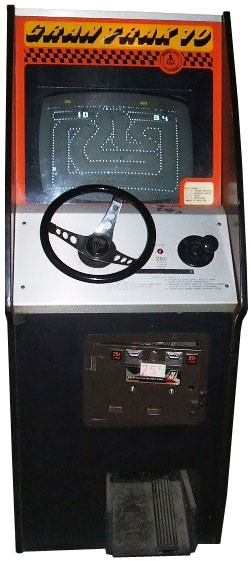
\includegraphics[scale=.33]{Arcade1} 
\caption{A photo of the Atari Gran Trak 10 from 1974, the first arcade vehicle. }
\label{fig:Arcade}
\end{figure}
\bigskip

None of the major motion capture game systems (such as the Wii, Playstation Move, Xbox Kinect) comes with a steering-wheel contraption specifically usable for vehicle-oriented games such as racing games. However, there are several examples of console enhancements that will allow the player to incorporate the steering wheel into their game style, enhancing the game-experience and unlock the natural feeling of controlling, most often, a motorized vehicle.
\bigskip

Where the Wii offers a solution that is compatible with the standard controllers, the X-Box 360 Kinect requires the purchase of an additional controller, which is steering-wheel shaped. Important to note is, that the steering wheel is an independent controller, hence it is does not interact with the Kinect camera. For this particular reason it rather resembles earlier generations of console/PC-steering wheel-controllers, neither which relied on motion tracking by camera.
\bigskip

In between the two is the PlayStation Move Racing Wheel, which is a hybrid of both the Nintendo Wii – and the Kinect steering wheel. Like the Wii, the Move Racing Wheel utilizes the preexisting game-controller, but includes additional functions/relocation of buttons, haptic feedback through vibration, to optimize the game experience.

\subsubsection{Steering wheel functionalities}
\subsubsection*{Introduction}
To account for the functionalities and usage of the controllers, this section covers the remote functionalities of the Wii controller, the Xbox 360 wheel controller and the PlayStation Move wheel controller. This information will make it possible to delimit the functionalities of the games that are developed to that specific console, and therefore controller, since there can only be as much functionality as the controllers support, in terms of buttons and/or motion control as there is available to the specific controller.

\begin{figure}[h] 
\centering
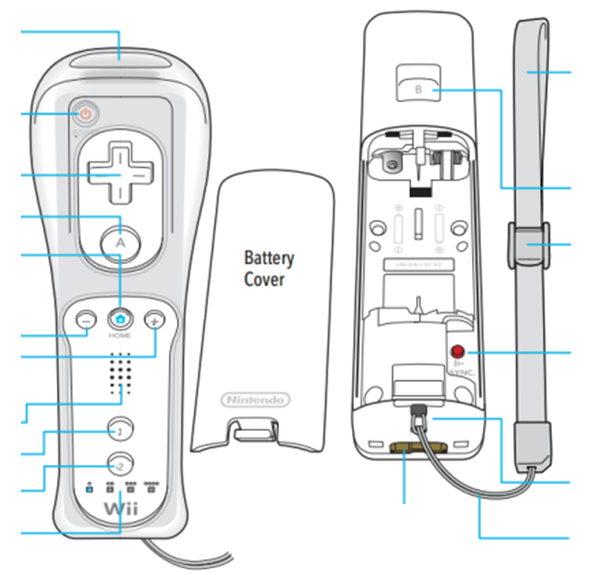
\includegraphics[scale=1]{WiiWheel} 
\caption{Wii Wheel}
\label{fig:Wiimote}
\end{figure}
\bigskip

\subsubsection*{Wii Wheel}
\parencite{Nintendo2013}\newline
As seen on Figure \ref{fig:Wiimote}. the Wii remote functionalities are listed in terms of functionalities and components. The Wii remote is mostly controlled through movement and gestures, so there is only a limited amount of buttons. Being:
\begin{itemize}
\item Control pad (Up, Down, Left, Right)
\item Pointer lens (the method for registering the controller movement)
\item A. \& B. Button
\item Home Button
\item Minus, Plus button
\item 1. \& 2. Button
\end{itemize}
\bigskip

\begin{figure}[h] 
\centering
\caption{Xbox wheel controller description (Danish)}
\label{fig:XboxWheel}
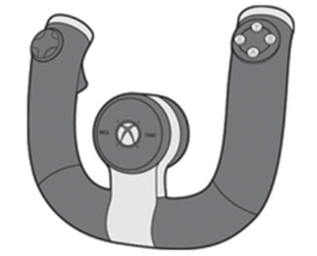
\includegraphics[scale=.75]{XboxWheel} 
\end{figure}
\begin{figure}[h]
\centering
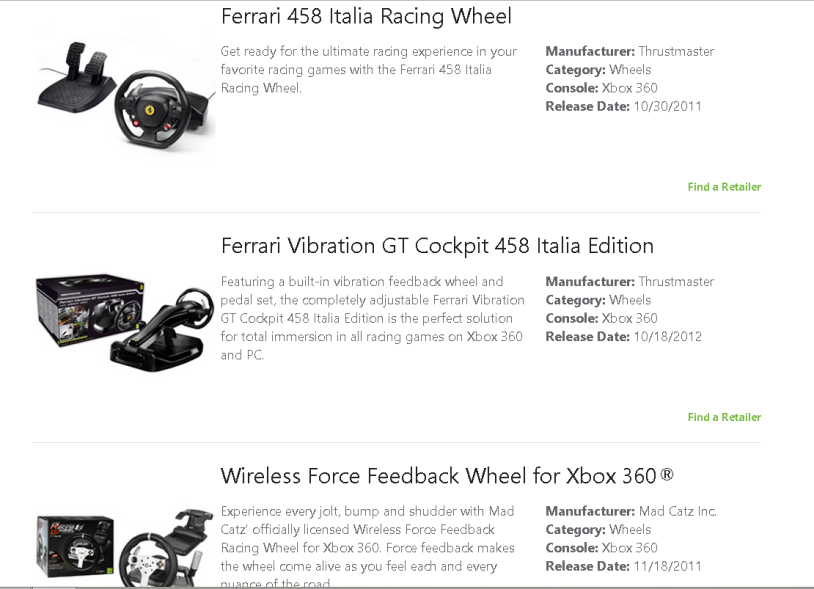
\includegraphics[scale=1]{XboxWheel2}
\caption{Xbox vehicle game controllers}
\label{fig:XboxWheel2}
\end{figure}

\subsubsection*{Xbox 360 wheel controllers}
\parencite{Xbox2013}\newline
As described on figure \ref{fig:XboxWheel}. The Xbox wireless Speed Wheel contains the following features and functionalities:

\begin{itemize}
\item Vibrating feedback
\item Movement tracking sensors
\item Release buttons for acceleration and braking
\item Buttons for game-defined functionalities (Standard Xbox controller functionalities)
	\begin{itemize}
		\item Buttons: A,B,X,Y
		\item Navigation-Button (left, right, up, down)
		\item Guide, start, back ( console control buttons)
	\end{itemize}
\end{itemize}

In addition, there are numerous steering wheel controllers compatible with Xbox that utilizes the same as above mentioned functionalities, but also included features such as floor pedals (throttle, brake, clutch) along with gear controller. See figure \ref{fig:XboxWheel2}. for a list of examples.
\bigskip

\begin{figure}[h]
\centering
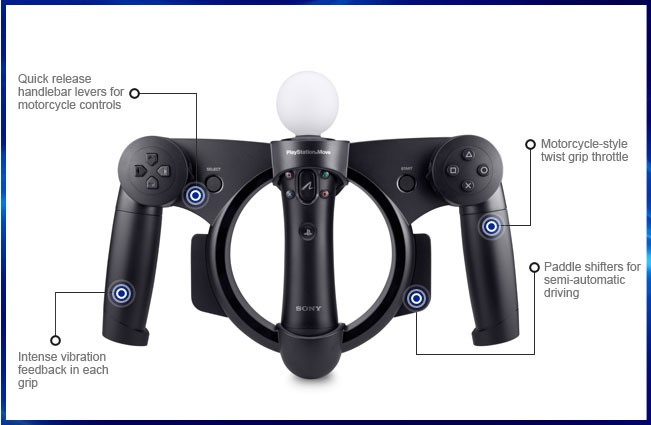
\includegraphics[scale=.5]{MoveWheel}
\caption{PlayStation Move Racing Wheel functionalities}
\label{fig:MoveWheel}
\end{figure}


\subsubsection*{PlayStation Move wheel controllers}
\parencite{Move2013}\newline
As seen on figure \ref{fig:MoveWheel}. The functionalities of the controller are as followed:

\begin{itemize}
\item Vibrating feedback
\item Movement tracking sensors
\item Quick release handlebar levers for motorcycle controls
\item Paddle shifters for semi-automatic driving
\item Buttons for game-defined functionalities (Standard PlayStation controller functionalities)
	\begin{itemize}
	\item Buttons: square, triangle, circle, cross
	\item Navigation-Button (left,right,up,down)
	\item Start \& Select ( console control buttons)
	\end{itemize}
\end{itemize}

\subsubsection*{Summary}
This section describes how the steering wheel controller has been developed to resemble a more realistic and intuitive experience when engaging in vehicle based gameplay. There is also accounted for the design in terms of functionalities of the Wii wheel controller, Xbox 360 wheel controller and PlayStation wheel controllers. This section covers the buttons and other controls of each controller to delimit the plausible amount of functionalities that can be implemented in possible gameplay with each controller.
\subsection{Game controls in various racing games}
\label{gamecontrols}
Within the State Of The Art of the formulated (IPS) area, we have to find out which choices are popular when it comes to deciding how you should be able to control your racing car in the game. This is needed in order to determine which requirements there are to the design of the controller, so that the user will be able to do the same actions in the game, as he/she would be able to perform in the same game played using e.g. Wii or Kinect.

By looking into which games in the racing category are popular on the three gaming platforms Nintendo Wii, Xbox Kinect and PlayStation Move, we can quickly see a difference in the supplies of racing games for the different platforms. It seems that finding a racing game for PlayStation Move is pretty difficult and the most prominent racing game designed for use with PS Move seems to be the game: \textbf{LittleBigPlanet™ Karting} \parencite{Miller2012}. Moving on to the Xbox Kinect; here it also seems that there is only one game standing when looking for the most popular racing game designed for the Kinect without the use of additional controllers, i.e. \textbf{Kinect Joy Ride}\parencite{Davidson2010}. Nintendo Wii, on the other hand, seems to be the most popular gaming platform of the three if you want to play a car racing game. For the Wii there are several different racing games that seem to be popular. Amongst those, we have various versions of \textbf{Need for Speed}, \textbf{TrackMania: Build To Race} and \textbf{Mario Kart Wii}, and \textbf{Sonic \& SEGA All-Stars Racing}, which looks much like Mario Kart in the controls. (This will be explained below) \parencite{Ign2013}.
In order to establish a general rule to follow when you want to create a controller that should be usable with most of the racing games available, a list of the different controls used by the games needs to be made. Making the foundation using the aforementioned 5 games we can assemble the following list:

Consistent for all five games:
\begin{itemize}
\item Steering left and right
\item Acceleration
\item Braking / Reversing
\item Changing camera view (at least for the Wii games - different views from game to game)
\item Display a pause menu
\end{itemize}

Need For Speed (Wii):
\begin{itemize}
\item Nitro (speed boost)
\item Change gear up and down
\end{itemize}

TrackMania (Wii):
\begin{itemize}
\item Braking while accelerating (Drifting)
\end{itemize}

Mario Kart Wii:
\begin{itemize}
\item Choose item
\item Throw items back and forward
\item Perform mid-air tricks
\end{itemize}

LittleBigPlanet™ Karting (Move):
\begin{itemize}
\item Use weapons
\end{itemize}

Kinect Joy Ride (Kinect):
\begin{itemize}
\item Charge and release speed boost
\item Drift to either side
\item Use item
\item Perform mid-air tricks in different directions
\end{itemize}

From this list, it can be seen that there are some general controls that are used through all of these different games. This means that when designing some form of game controller for a car racing game, you should make the user able to perform the five commands listed at the top, as those commands seem to be important, when they are consistent through multiple games. Furthermore, depending on what game we are talking about, there seems to be about 1 – 4 additional controls to be able to play the game fully.


\subsection{Visual Computing}
Visual Computing is computing, which lets the user interact with, and/or control work by manipulating visual images \parencite{Rouse2013}. The visual images can be photographs, 3D-scenes, video sequences or any other visual output for that matter.

It is the core of controlling and manipulating images and is therefore an important aspect to include in the research and find already established solutions to this method.
\bigskip

One example of Visual Computing, which is developed for the PC, is Camspace\copyright. Camspace is a platform for visual computing that, through the use of a standard webcam, detects object and hand gestures and then utilize those to be implemented in games, as a mouse controller etc. \parencite{Camspace2009}

It works as a software platform that is installed on any computer with access to a basic webcam, where options to determine the use dictates how the user interacts with it through human gestures with or without an object.
\bigskip

The program can utilize an object as a controller by presenting a solid object with a uniform color that does not match the environment i.e. the shirt that is worn or the wall behind the player. Also, the room must be well lit for the color recognition to be possible.
\bigskip

Camspace offers games and programs that are specifically designed for the software itself, but does also contain drivers for it to be compatible with pre-existing games, which is developed with other means of control. Although the games are compatible with the software, it is only a limited amount of controls that can be implemented to function with the program.

\begin{table}[h]
\begin{tabular}{| l | l }
Game Title & In-game functionalities\\
\hline \hline
Need for speed underground 2 & Move left/right \& accelerate/break\\
Aquadelic & Left/right \& horizontal\\
Trackmania (\& Nations) & Speed (depth of object) \& left/right\\
LudoRace & Left/right\\
OffRoadArena & Speed(depth of object) \& left/right\\
Flight Model Simulator & N/A\\
Need for speed Carbon & N/A\\
\end{tabular}
\caption{List of vehicle based (driving, sailing, flying) games and the in-game functionalities which is utilized by the Camspace software\parencite{Camspace2009}}
\label{tab:camspace}
\end{table}

\subsubsection*{Summary}
The research indicates that it is possible to create software for computers that utilizes simple webcams for visual computing purposes, such as game control and interaction. It is also possible to modify the use of the program in order to access and control games which is not specifically developed for Camspace itself. Although it is possible, it is only a limited amount of controls that can be imported and utilized via Camspace; (See table \ref{tab:camspace})  such as speed increase/decrease by pulling the designated control object closer or further away, and turn/rotation by rotating the object left or right.
\subsection{Image and video processing}
Because of the initial naive designs, it was determined that image or video processing would be needed to be researched for finding the position of different elements. In this section, methods for detecting objects in an image are therefore being researched. It is necessary to figure out how to detect certain objects in the scene, to use it for controlling things in games or other interactive media.

\subsubsection{Color detection}
A very simple and useful way of detecting objects in a scene, is by using color detection. The drawbacks of this are that it is sometimes necessary to put certain colors on objects that will be used in the scene, in order to make them easier to detect. It is also a good idea to have a background with very few colors, so the colors are easier to seperate. It can limit the colors the user can wear, for example if the camera is set to detect green colours and the user is wearing a green shirt. For example, if an image is searched for green colors, and the user is wearing green, the program will always detect the user. While this might be exactly what the program should do, it would be a benefit to be able to control what to detect, and not just give in to randomness.

To enable color detection, thresholding can be used. Thresholding is isolation of a color or a spectrum of colors. For example, to isolate objects that are very red, the statement r > 200 could be used. This would isolate all colors with a red value greater than 200, turning them white in the output image. Here is a simple example on how to use thresholding, written in pseudo-code. This is assuming the input is an RGB image, and the output is a grayscale image.

\begin{algorithm}[H]
\caption{Color thresholding}
\label{code:threshold}
\begin{algorithmic}
\IF {$ R>R_{min} \; and \; R<R_{max} \; and $\\
	 $ G>G_{min} \; and \; G<G_{max} \; and $\\
	 $ B>B_{min} \; and \; B<B_{max}$\\}
\STATE $g(x,y)=255$
\ELSE
\STATE $g(x,y = 0$
\ENDIF
\end{algorithmic}
\end{algorithm}

In the above example, R, G, and B stand for red, green and blue, and g(x, y) is the output image, where the x and y is the position of the pixel current being processed. For most computers and image acquisition, the RGB color space is used, hence the lack of detail about how to use any other color spaces. In the Gesture Recognition chapter, other color spaces will be discussed, as they make more sense in that situation. The output of the above code would be a binary image. For each pixel in a binary image, it can only have two different values: 0 or 255. This ensures that it is easier for the program to work with, as it only have to compare two values, not 256 values.

Isolating a certain color isn’t enough to actually do something with it though. If one wishes to figure out what position a colored object is at, it is a good idea to find the average center of the detected color. A way of doing this by finding the average position of all the white pixels in the output image. So, for each white pixel, add its x and y position to one variable each, and have another variable that counts how many white pixels there are. Then, divide all the x values added together with the number of pixels, and do the same for all the y values.

The computer now knows the average position of a certain color in the scene. But what if the program should detect more colors? One way of doing this, is to avoid using a binary image for the output, and instead have the output be of many different values and or colors. Each thresholded color then has their own color in the output.

\subsubsection{BLOB analysis} \label{sec:blob}
BLOB stands for \textbf{B}inary \textbf{L}arge \textbf{OB}ject, and in image processing it represents a group of white or black pixels. As mentioned above, it’s possible to detect several colors by having several colors in the output as well. This however means that the program can’t actually separate several objects of the same color. To fix this, a BLOB analysis could be used. To separate each BLOB, a so-called grassfire algorithm 
\footnote{A grassfire algorithm is an algorithm that detects and separates all BLOBs in a scene, by finding a detected pixel, and then labeling all connected pixels as one BLOB (also known as “burning” the pixels).} 
is usually used, with either 4- or 8-connectivity \parencite{Moeslund2012}. 4-connectivity checks the pixels above, below, to the left and to the right of the current pixel, whereas 8-connectivity also checks the pixels diagonally from the current pixel. 8-connectivity is more precise in a sense, since it’s able to detect small diagonal lines unlike 4-connectivity, but it takes more processing power.
\bigskip

The recursive grassfire algorithm, which is usually considered the normal grassfire algorithm, “burns” every white pixel in an image, where the white pixels represent something that has been detected. When the program searches through the image and encounters a white pixel, it’ll run a function containing the grassfire algorithm. This algorithm changes the white pixel to a gray pixel, with a value of 1-254. By doing this, the pixel is “labeled” with a number from 1-254, so the program can find these labeled pixels later. The reason we can’t use numbers below 1, is because that would label the pixel as being black, which the program ignores, and it can’t be labeled above 254, because the program detects it as something white which is has to make computations on, creating an infinite loop.

After labeling, the function will check if there is another white pixel next to the one it just marked. If there is, it’ll label that pixel with the same label as the one before (it will “burn” the pixel), and check if there are any white pixels next to that one. It’s called a recursive function, since it references itself. This continues until the function can’t find any more white pixels connected.
By doing this the program labels each white “island” of pixels, so it is easier to separate them and analyze each BLOB alone.

Note that there is also a sequential grassfire algorithm, which in some cases is more safe to use than the recursive one, since it doesn’t risk running out of memory in the same way as the recursive. The computer only has a limited amount of memory allocated for function calls, and since the recursive function calls itself multiple times, it risks running out of memory if it encounters a very large BLOB, whereas the sequential algorithm doesn’t call itself, and as such doesn’t risk running out of memory. \parencite{Moeslund2012}

\subsubsection{Background Subtraction} \label{sec:BGSub}
The theory behind detecting changes in video is to have a reference image, and subtract that from the recorded image. This effectively removes the background in the image, and leaves only whatever change has been made in the picture. It is also necessary have to perform thresholding, and filter any noise away.

\subsubsection{Other detection methods}
There exist a lot of other ways to detect something in an image or a video feed, for example it might be necessary to detect how much something is rotated, which in turn could require template matching or other methods to find a certain object with a certain pattern.

It can also be useful to be able to track something in a video feed. Arguably some might say that video tracking has already been described in this research, since detecting a certain color for each frame can be interpreted as “tracking” that color \parencite{Moeslund2012}, however that is not necessarily true. In order to actually track something, the program needs to be able to predict where the point it’s trying to track will go to in the next frame. Being as many cameras today run at 24-60 frames per second (fps), an object can’t move too far in an image unless it’s travelling at extremely high speeds.

\subsubsection{Summary}
Color detection is achieved by using thresholding, which isolates certain colors so they can be detected. Color detection is useful if the program only needs to detect one color, or if it needs to detect more than one easily detectable color (for example detection of red, green and blue, in an otherwise white scene).

However if for example a program is required to detect two different players in a two player game, where each player is holding up a red sticker for detection, the program needs to separate these two colors. This is where BLOB detection comes in use, by detecting each BLOB of white pixels, by using a grassfire algorithm. Note that BLOB detection can be used in turn with almost any other detection method, in order to separate objects in the scene.

If the program needs to detect objects that enter a scene, the program can have a reference image of the scene without any objects, and then subtract that image from the video feed. Anything that enters will then stand out. \parencite{Moeslund2012}

\subsection{Gesture Recognition}
The concept is focused on using the user as the controller and letting the movements of the user dictate how the computer should react. In order to accomplish this, knowledge of know how to make the computer understand the user’s intended action is needed. Since the concept will be camera based, the proper tool for reading a user is gesture recognition.
\bigskip

\begin{figure}[h] 
\centering
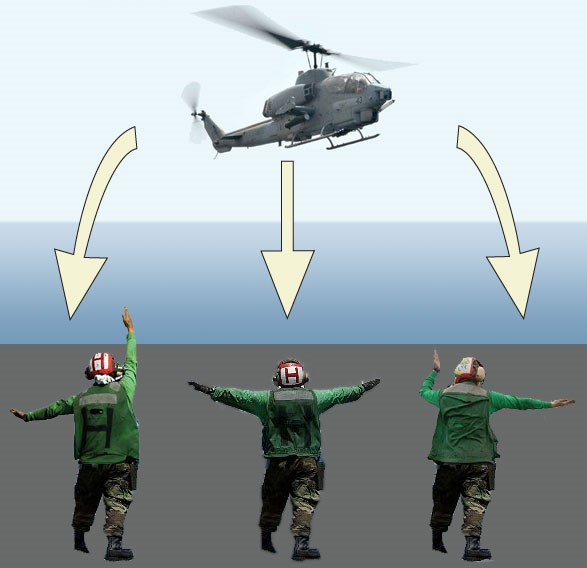
\includegraphics[scale=.33]{Gesture1} 
\caption{Gestures used to communicate instructions to a helicopter.}
\label{fig:Gesture1}
\end{figure}

\subsubsection*{What a gesture is and what they mean in relation to the concept.}
The common dictionary defines a gesture as: \textit{“a movement that communicates a feeling or instruction […]”} and \textit{“to make a movement with your hands or head in order to show or tell someone something […]”}. \parencite{Macmillan2005}
This means that a general gesture is used as a form of speechless communication between two parties used to relay a message or an intent, as seen in Figure \ref{fig:Gesture1} where a movement command is being relayed to a helicopter. Gestures is often used when speech is difficult or impossible.

Because the solution will be based on a camera, then gestures will be the only viable way to communicate an intended action to the computer. Within the scope of the concept, this means that a gesture is a movement, primarily using arms or torso, which communicates an instruction to a computer to be used in an application.
\bigskip

Secondly it is necessary to know how to make a computer understand gestures given to it. For this, image processing is needed.

The first thing that needs to be done to an image of a gesture is to isolate the gesture from the rest of the image. Some methods of doing this includes background subtraction and hue based extraction based on the hue of human skin \parencite{Busaryev}.
\bigskip

Background subtraction \footnote{section: \ref{sec:BGSub}} uses the mean values of a series of images of the same background as a basis for subtracting objects from new images. If a pixel in a new image is different enough from the mean value of the series, then the pixel can be used in a binary image of the objects. The problem with this approach is that variable conditions like lighting and noise can corrupt the results by creating false positives or objects with wrong properties. \parencite{Busaryev}
\bigskip

Another approach is hue based extraction, which converts the image to the HSV (hue, saturation, and value) color space and then uses thresholding to detect human skin in the image. Caucasian skin has a very distinguishable hue values, which make it easier to detect through hue rather than regular RGB. \parencite{Busaryev}
\bigskip

A method of recognizing the gesture is the Local Feature Classifier method \parencite{Busaryev}, which uses the contours of a hand and points along the contour to distinguish for example one shown finger from two and other gestures. With adjustments, this method can be used on bodies and other features.

\subsubsection*{Summary}
In summary a gesture is a movement used to communicate an instruction to a computer to be used in an application. Background subtraction or hue based subtraction, based on the hue of the skin of the user, can be used to extract a gesture from an image. The Local Feature Classifier method can be used to translate the gesture to an application command.
\subsection{User Control Experience}
The focus in this project is to make a controller that is based on the user’s gestures and movements. In order to accomplish that kind of controller a lot of research is required on how the movements has to be executed in order to make it a smooth and positive experience for the user. If this project wants to achieve that feeling it needs research about how the human body communicates by the use of body language. As body language is a huge subject, it has been chosen to only focus on the essentials of the subject and the relevant body parts for the webcam to detect.

In order to create gestures for the webcam to detect there has to be an understanding of what a gesture is. Many have asked this question and according to Adam Kendon an experiment were made with this goal in mind in the year 1978 \parencite{Kendon2004}:
\bigskip

\emph{"What are the features that an action must have for it to be treated as a gesture?"} \parencite{Kendon2004}
\bigskip

This experiment was performed by having twenty people with no psychology or behavioral science background. This background check was made to be sure that it would not have any impact on the test. The people was placed in rooms and told to watch a four minute movie clip without sound made for the experiment. After the movie was done each person was asked to describe what movements they had seen the man in the movie make. The aim was to find out what movements the subjects picked out in their descriptions and to find out what different sorts of movements they identified. After more tests and a lot research the scientists came to a conclusion.
\bigskip

\emph{“Gesture is a label for actions that have the features of manifest deliberate expressiveness. They are those actions or those aspects of another’s actions that, having these features, tend to be directly perceived as being under the guidance of the observed person’s voluntary control and being done for the purposes of expression rather than in the service of some practical aim.”} \parencite{Kendon2004}
\bigskip

As recording to the research, gestures have a huge impact on the listeners. Even though webcams do not have any ears these theories can still be of use for us. As Susan Goldin-Meadow writes in her book \parencite{Meadow2005} people still use gestures even though they are not communicating with another person. This could be you at home practicing a speech or simple just talking to yourself. You talk but even if you are the only one in the room you would still perform your gestures, as you were trying to explain something to another person.

Now that it is known what a gesture is, the research can continue on which gestures needs to be implemented. A few common gestures have been found that are being used in the daily lives that could be useable for the webcam to detect \parencite{Businessballs}.
\bigskip

Common gestures:

Hands:
\begin{itemize}
\item Thumb up - positive approval, agreement, all well
\item Thumb down - disapproval, failure
\item Index finger and thumb touching at tips - satisfaction
\end{itemize}

Head:
\begin{itemize}
\item Head nodding - agreement
\item Head shaking - disagreement
\end{itemize}
\bigskip

A last thing of mention is that people has a personal space also called Proxemics with five different comfort zones. close intimate, intimate, personal, social-consultative and public. All of these zones define how comfortable the person is with another person standing around them. So this is something that should be kept in mind when creating the controller. If the aim will be for the Social-consultative and Public zone. It is then important according to Edward Twitchell Hall that we place cameras and other players at least 1.2 meters away from the player in order for the person to feel comfortable between themselves and others \parencite{Businessballs}.

So what can be concluded from this research is that in order to make a good controller that is based on the user’s gestures and movements. A test has to be made in order to show how people want to handle the different movements and actions that the webcam will observe. With the information received from the initial tests it is then possible to create a pattern that fits the majority of volunteers used for initial testing. After that it should be possible to implement the right movements and gestures for the controller and then give the right instructions for our movements at the final test.  This process should make it a smooth and positive experience to use the controller created for the project.


\subsection{Analysis summary}
From the analysis, some key elements were found, in regards to the initial problem statement, and how to create a solution for the problem.

The first point that becomes apparent is that while the initial problem statement is technically solved by using Camspace, it also proves to be insufficient for the desired use, as the controls are limited to movement, and not special actions. This is further emphasized as a problem when looking at the fact, that none of the researched racing games make do with simply movement, they all have one or more additional features, which are essential for the game play.

Another important section of knowledge gained from the analysis, is the different ways to create the program. The analysis shows different methods of doing it, and gives arguments for how each method could be used, which will help deciding, when the product is going to be designed.
From the analysis, the initial problem statement can be modified, and turned into a final problem statement, on which the continuing project can be based.

\subsection{Final problem statement}
Can a vehicle game controller be created, using a standard web cam that utilizes visual computing with functionalities, that are comparable to state of the art game controllers in terms of functionality?